\documentclass[a4paper,12pt]{article}

\usepackage{listing}
\usepackage{graphicx}

\begin{document}


\title{7. Implementation of client server communication using socket programming and TCP as transport layer protocol}
\author{Santhisenan A}
\date{\today}
\maketitle

\section{Socket Programming}

\subsection{Socket}
A socket is one of the most fundamental technologies of computer network programming. Sockets allow network software applications to communicate using standard mechanisms built into network hardware and operating systems.


A socket represents a single connection between exactly two pieces of software (a so-called point-to-point connection). More than two pieces of software can communicate with client/server or distributed systems by using multiple sockets. For example, many Web browsers can simultaneously communicate with a single Web server via a group of sockets made on the server.


Socket-based software usually runs on two separate computers on the network, but sockets can also be used to communicate locally (interprocess) on a single computer. Sockets are bidirectional, meaning that either side of the connection is capable of both sending and receiving data. Sometimes the one application that initiates communication is termed the "client" and the other application the "server," but this terminology leads to confusion in peer to peer networking and should generally be avoided.

\subsection{Socket Interface Types}

Socket interfaces can be divided into three categories:

\begin{itemize}
	\item \textit{Stream sockets}, the most common type, requires that the two communicating parties first establish a socket connection, after which any data passed through that connection will be guaranteed to arrive in the same order in which it was sent - so-called connection-oriented programming model.
	\item \textit{Datagram sockets} offer "connection-less" semantics. With datagrams, connections are implicit rather than explicit as with streams. Either party simply sends datagrams as needed and waits for the other to respond; messages can be lost in transmission or received out of order, but it is the application's responsibility and not the sockets to deal with these problems. Implementing datagram sockets can give some applications a performance boost and additional flexibility compared to using stream sockets, justifying their use in some situations.
	\item The third type of socket -- \textit{the raw socket} -- bypasses the library's built-in support for standard protocols like TCP and UDP. Raw sockets are used for custom low-level protocol development.
\end{itemize}

\subsection{Socket support in network protocols}
Modern network sockets are typically used in conjunction with the Internet protocols -- IP, TCP, and UDP. Libraries implementing sockets for Internet Protocol use TCP for streams, UDP for datagrams, and IP itself for raw sockets.


To communicate over the Internet, IP socket libraries use the IP address to identify specific computers. Many parts of the Internet work with naming services, so that the users and socket programmers can work with computers by name (e.g., "thiscomputer.wireless.about.com") instead of by address (e.g., 208.185.127.40).


Stream and datagram sockets also use IP port numbers to distinguish multiple applications from each other. For example, Web browsers on the Internet know to use port 80 as the default for socket communications with Web servers.


\section{TCP}
The Transmission Control Protocol (TCP) is one of the main protocols of the Internet protocol suite. It originated in the initial network implementation in which it complemented the Internet Protocol (IP). Therefore, the entire suite is commonly referred to as TCP/IP. TCP provides reliable, ordered, and error-checked delivery of a stream of octets (bytes) between applications running on hosts communicating by an IP network. Major Internet applications such as the World Wide Web, email, remote administration, and file transfer rely on TCP. Applications that do not require reliable data stream service may use the User Datagram Protocol (UDP), which provides a connectionless datagram service that emphasizes reduced latency over reliability.

\section{Code} 
\subsection{client.py}
\begin{verbatim}
# client
import socket

# create a socket object
s = socket.socket(socket.AF_INET, socket.SOCK_STREAM)

# get a local machine name
host = socket.gethostname()
port = 9999

# connection to hostname on port
s.connect((host, port)) 

# recieve no more than 1024 bytes
tm = s.recv(1024)

s.close()

print("Time got from the server is %s" % tm.decode('ascii'))
\end{verbatim}
\subsection{server.py}
\begin{verbatim}
import socket
import time

# create a socket object
ServerSocket = socket.socket(socket.AF_INET, socket.SOCK_DGRAM)

# get local machine name
host = socket.gethostname()
port = 9999

# bind to the port
ServerSocket.bind((host, port))

ServerSocket.listen(5)

while True:
    # establish a connection
    ClientSocket, addr = ServerSocket.accept()

    print("Got a connection from %s" % str(addr))
    CurrentTime = time.ctime(time.time()) + "\r\n"
    ClientSocket.send(CurrentTime.encode('ascii'))
    ClientSocket.close()
\end{verbatim}

\section{Output}

\pagebreak
\begin{figure}
	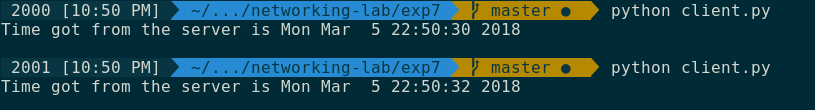
\includegraphics[width=\linewidth]{./tcp-client.png}
	\caption{Client}
	\label{fig:client}
\end{figure}

\begin{figure}
	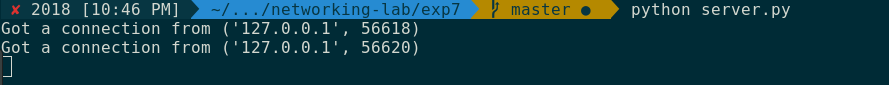
\includegraphics[width=\linewidth]{tcp-server.png}
	\caption{Server}
	\label{fig:server}
\end{figure}


\end{document}